\documentclass[12pt,letterpaper]{article}
%\usepackage{preamble}

%\ProvidesPackage{preamble}

\usepackage{fullpage}
\usepackage[top=2cm, bottom=4.5cm, left=2.5cm, right=2.5cm]{geometry}
\usepackage{amsmath,amsthm,amsfonts,amssymb,amscd}
\usepackage{lastpage}
\usepackage{enumerate}
\usepackage{fancyhdr}
\usepackage{mathrsfs}
\usepackage{xcolor}
\usepackage{graphicx}
\usepackage{listings}
\usepackage{hyperref}
\usepackage{enumitem}
\usepackage{float}
\usepackage{fancyvrb}
\usepackage{color,soul}
\sethlcolor{lightgray}
 \usepackage{subfigure}
 \usepackage{textcomp}
\usepackage{siunitx}

\usepackage{graphicx}
\usepackage{array}

\usepackage[T1]{fontenc}
\usepackage[numbered,framed]{matlab-prettifier}
\hypersetup{%
  colorlinks=true,
  linkcolor=blue,
  linkbordercolor={0 0 1}
}

\let\ph\mlplaceholder % shorter macro
\lstMakeShortInline"

\lstset{
  style              = Matlab-editor,
  basicstyle         = \mlttfamily \small,
  escapechar         = ",
  mlshowsectionrules = true,
  xleftmargin=.01\textwidth, xrightmargin=.01\textwidth
}

\graphicspath{{./problem1_images}}

\pagestyle{fancyplain}
\headheight 35pt
\lhead{\userID}
\chead{\textbf{\Large Project \hwnumber}}
\rhead{\course \\ \today}
\lfoot{}
\cfoot{}
\rfoot{\small\thepage}
\headsep 1.5em




%%%%%%%%%%%%%%%%%%%%%%%%%%%%%%%%%%%%%%%%%%
%%%% Edit These for yourself
%%%%%%%%%%%%%%%%%%%%%%%%%%%%%%%%%%%%%%%%%%
\newcommand\course{Econ 672}
\newcommand\hwnumber{2}
\newcommand\userID{Ziming Huang}
\newenvironment{alphaparts}[0]{%
  \begin{enumerate}[label=\textbf{\Alph*}]
}{\end{enumerate}}


\begin{document}
%\textbf{\Large PROJECT 1}



 




\section*{Exercise 1}
  \begin{enumerate}[label=\textbf{(\Alph*)}]
%----A-----
  \item Interprets of parameters:\\
 	 \begin{enumerate}[label=(\roman*)]
  	    \item We can use the function \hl{datevec} to get [Y,M,D,H,MN,S] of our data by inputting our dates and the date form (the input dates need to be strings) :
  	    
  	    \hl{datevec('dates','yyyymmdd hhmmss')}. \\
  	    
  	    
  	    We can also get  [Y,M,D,H,MN,S] by doing some calculations:
  	    
  	    \hl{Y=floor(dates(:,1)/10000);
  	    
  	        M=floor((dates(:,1)-Y*10000)/100);
  	        
  	        D=dates(:,1)-10000/*Y-100/*M;
  	        
  	        H=floor(data(:,2)/10000);
  	        
  	        MN=floor(data(:,2)-H/*10000)/100;
  	        
  	        S=data(:,2)-10000/*H-100/*MN}. 
  	        
  	    
  	  Given the data we have, the second method will cost less time since we do not need to change our data form(double) to strings which we will need to do if we want to use the first method.             
  	  
  	    \item We can store prices in either a matrix or a vector. Comparing to vector, storing prices in matrix makes it possible for us to group this data by day, which will be helpful for avoiding calculate overnight returns. What's more, store changing from matrix to vector is very simple by using the code: \hl{matrix(:)}.
  	    ~~\\
  	    
  	    
   The \textbf{MATLAB} code:
   \lstinputlisting{functions/load_stock.m}
   ~~\\
   
      \end{enumerate}	
      

 %----B-----
 \item From our data, we have:
 \begin{center}
 	 	\begin{align*}
 	 T_{PG}&=2769   ~~~~ N_{PG}=78\\
 	 T_{DIS}&=2769  ~~~~ N_{DIS}=78\\
 	    \end{align*}
     \end{center}
We can find the value of $N$ by count the number of values that equal to the first value in first column; We can find the value of $T$ by dividing the row size of our dates into N:

\hl{N=sum(dates(1,1)==dates(:,1));

n=N-1;

T=size(dates,1)/N;}
\\

%-------C-----------
\item 
   \begin{enumerate}[label=(\roman*)]
  	    \item The regular market time is from 09:30 a.m. to 4:00 p.m., so the market hour is 6.5 hours. 
  	    \item If the data is sampled every 5 minutes, that is $\Delta_n=5 minutes$, then the observation numbers every day is $N=\frac{1}{\Delta_n}+1=79$.
  	    \item The total number of observation is differ from the value in part(B);
  	    \item The reason of these differencse can be that since the open price may contain large noises, this will have a big influence on our calculation (especially for high frequency data). In order to cancel this effects, we always let out the open price from our data.\\
  	\end{enumerate}  

%-------D-----------
\item We can avoid calculating overnight returns by reshape our prices into group (by day); we can delete the date time of the first observation each day to construct a new date time matrix which is right for our log-return data. 

To extent the application of the function \hl{log\_return}, I have added two other parameters:

\textbf{\emph{N}}: is the number of observations our data provided every data. If N=78, then we will have 78 data every day; 

\textbf{\emph{J}}: is the number of steps(intervals) between every used observation. If J=1, means we will use all our data to do analysis; if J=10, means we will just pick 1th,11th,21th... observation data to do analysis.\\

The outputs of this function are return\_dates and log\_return(not in percentage), they are grouped by day and shown in matrix.

The \textbf{MATLAB} code:
   \lstinputlisting{functions/log_return.m}
   ~~\\
   
   
%-------E-----------
\item We first need to transfer the outputs of function \hl{log\_return} into vectors by using the code:  \hl{matrix(:)}, and then convert the log-return to percentage. The follows are the figures of price and log-return for PG and DIS:
 \begin{figure}[H]
           \subfigure{
           \begin{minipage}[l]{1\linewidth}
           \centering
            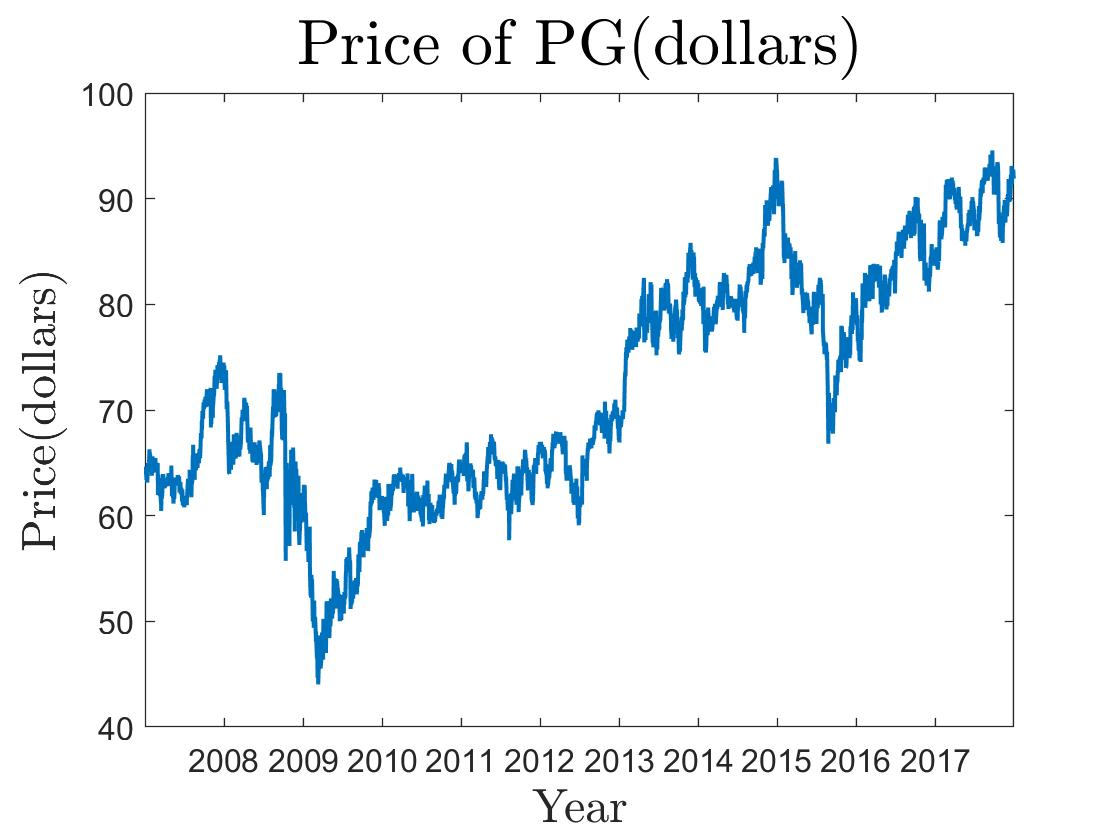
\includegraphics[width=3in]{figures/p2_ex1_e1_PG.jpg}
            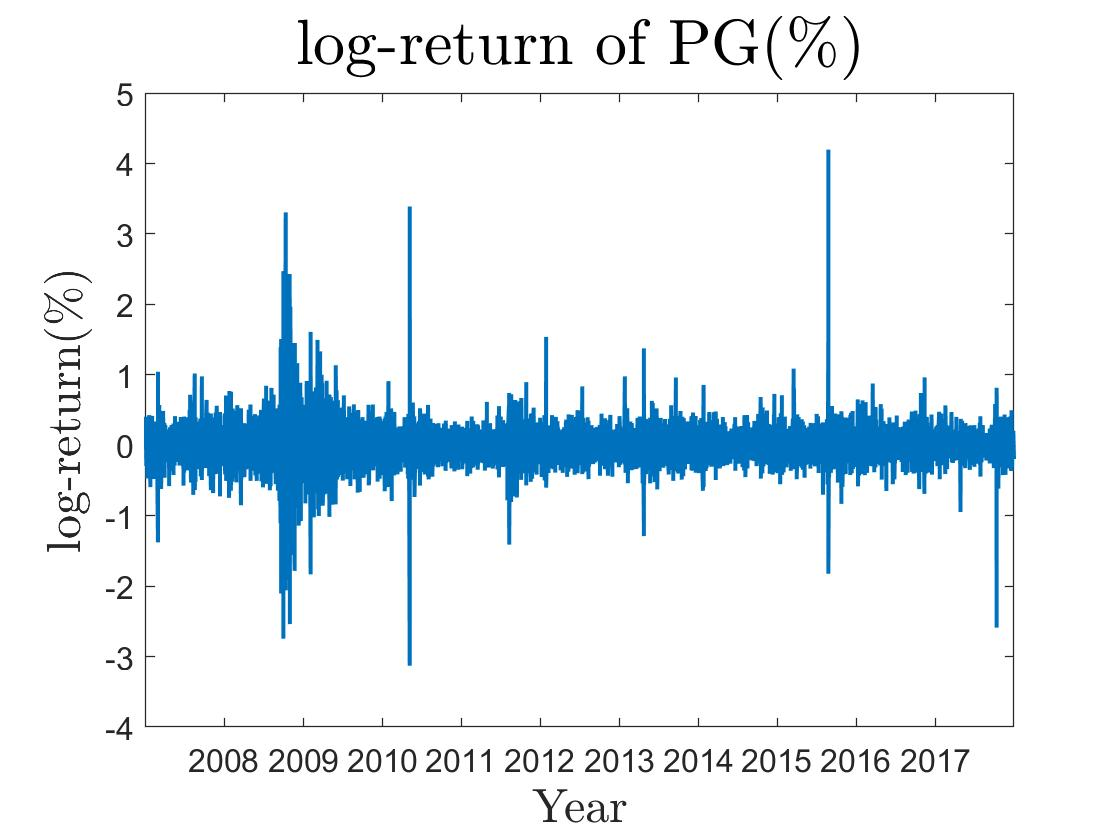
\includegraphics[width=3in]{figures/p2_ex1_e2_PG.jpg}
            \end{minipage}
            }
          \subfigure{
           \begin{minipage}[r]{1\linewidth}
           \centering
           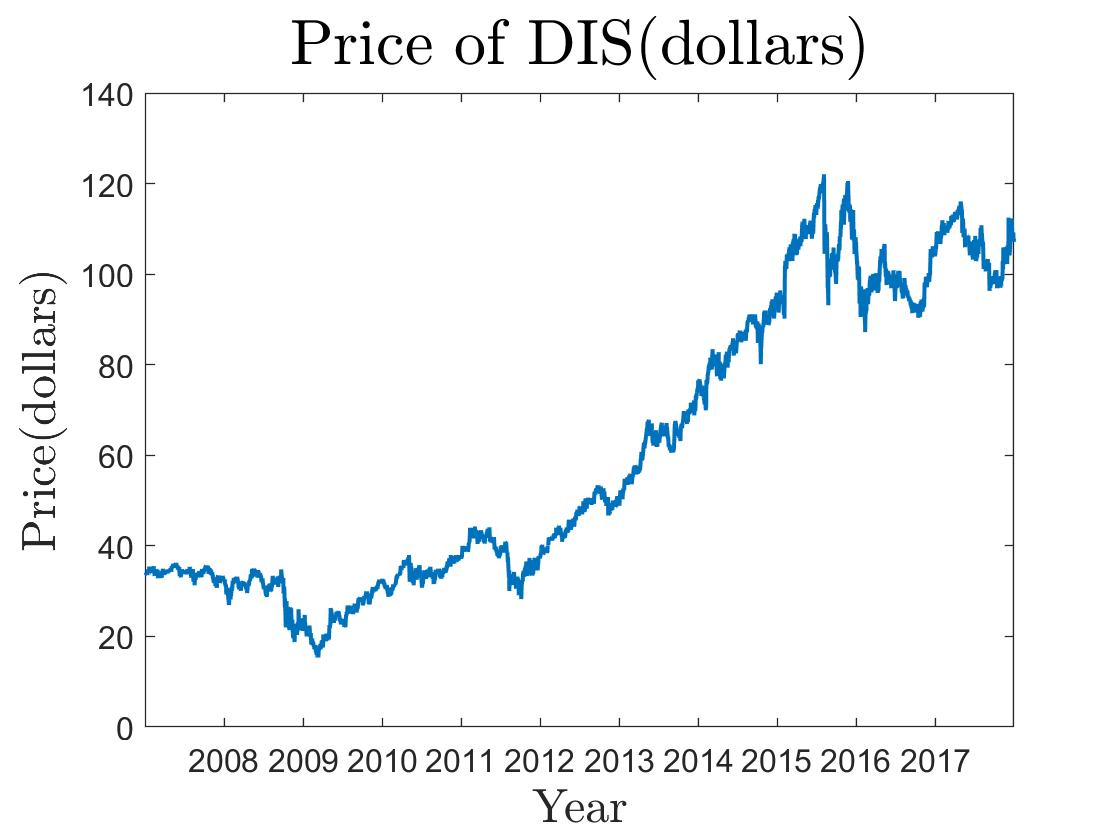
\includegraphics[width=3in]{figures/p2_ex1_e1_DIS.jpg}
            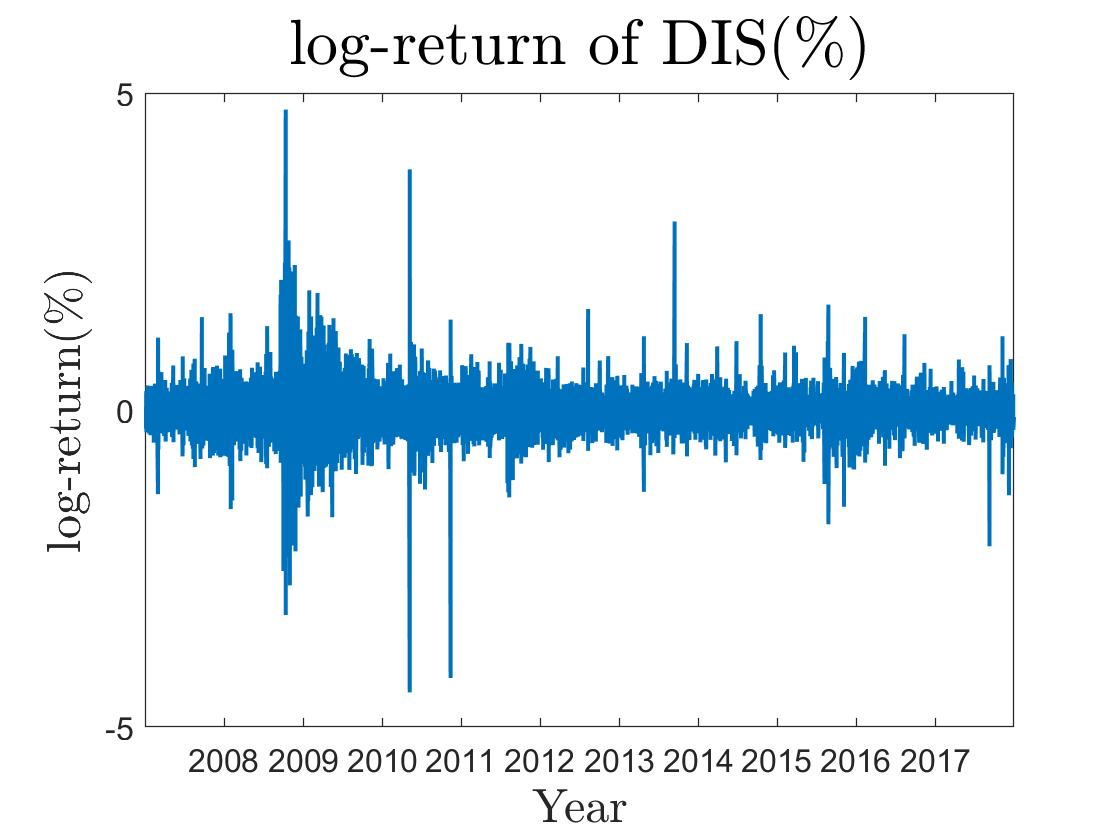
\includegraphics[width=3in]{figures/p2_ex1_e2_DIS.jpg}
            \end{minipage}
            }
            \centering
            \caption{Price and log-return}
\end{figure}

From the price figure, we can know the range of price for PG and DIS are (44\$,95\$) and (18\$,120\$) respectively. Even thought the price range for DIS' price is larger, PG's price shows more volatility. As we can see, PG's price went through a big fluctuation around 2009, median 2014 and median 2015.  
\\

From the log-return figures, we can find the both the log-returns of PG and DIS move around with 0. But we can also find that there are some abnormal values in both the PG and DIS' log-returns. For PG, it has three abnormal return: around 2009, median 2010 and median 2015; for DIS, there are 4 abnormal return: around 2009, 2010, 2011 and 2013. These abnormal returns show that our data may probably exist outliers. 
\\

%-------F-----------
\item 
 \begin{enumerate}[label=(\roman*)]
  \item Stock splits is the decision made by the board of company to increasing company outstanding share by issuing more stocks to current investors.
  \item By stock splits, the company's stock price decreases, so the stock price will become more attractive to potential investors. As a result, the liquidity of stock will increase. This is good for company to raise fund when they are needed.
  \item A company will choose stock splits when the stock price is too high to attractive potential investors to invest. A company can choose any time to split stocks through the whole year.
  \item Usually stock splits will lead to a decrements of stock price, so the log-return will show a downside jump.
  \item From the figure, we can find some downside jump of log-return, the time of these downside jumps are around the middle of the year, so there is a big chance that these jumps are caused by stock splits.
  \item Yes, they provide the adjusted price which has been adjusted for stock dividends or stock splits.
  \item No, stock price will affect the price begin the stock market hours, so it will not affect the return calculated within the day.\\
  \\
  
\end{enumerate}
The \textbf{MATLAB} code for Exercise 1(for PG):
   \lstinputlisting{scripts/p2_ex1_PG.m}

\end{enumerate}
\newpage

%---------------------------------------------

\section*{Exercise 2}
  \begin{enumerate}[label=\textbf{(\Alph*)}]
%----A-----
\item
Here are the figures of RV for PG and DIS:
 \begin{figure}[H]
           \subfigure{
           \begin{minipage}[l]{1\linewidth}
           \centering
             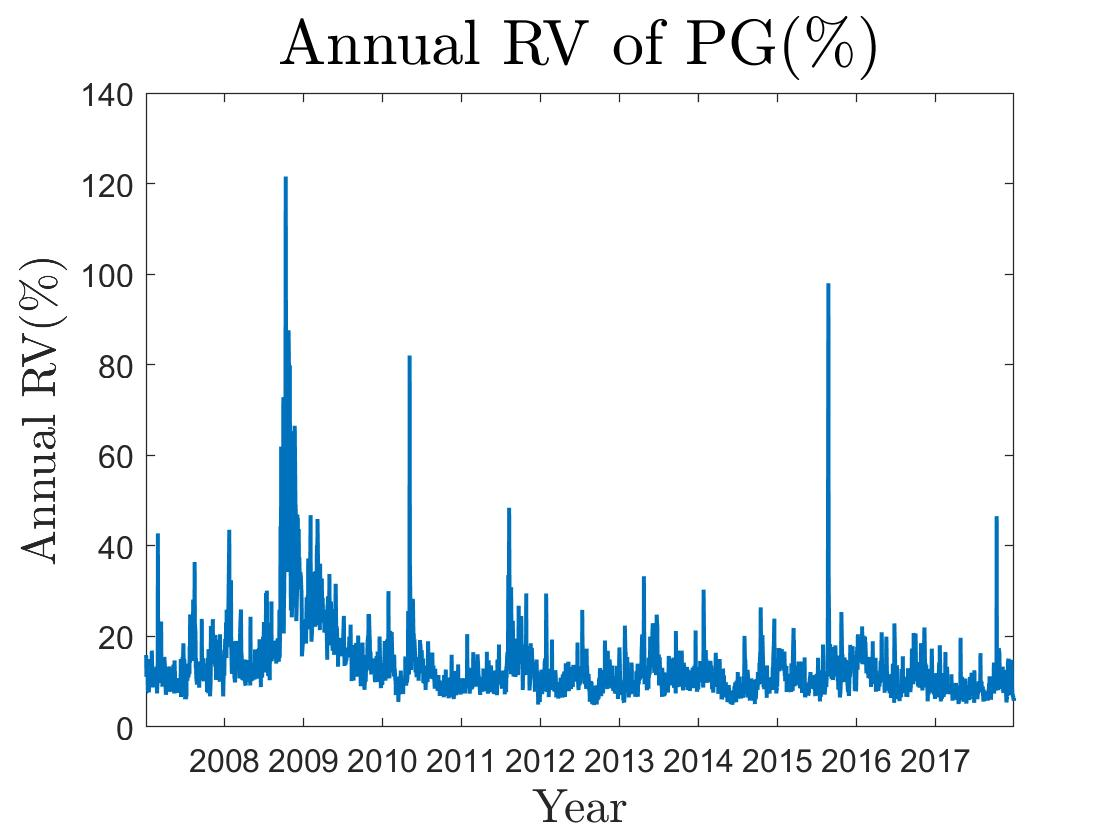
\includegraphics[width=3in]{figures/p2_ex2_a_PG.jpg}
              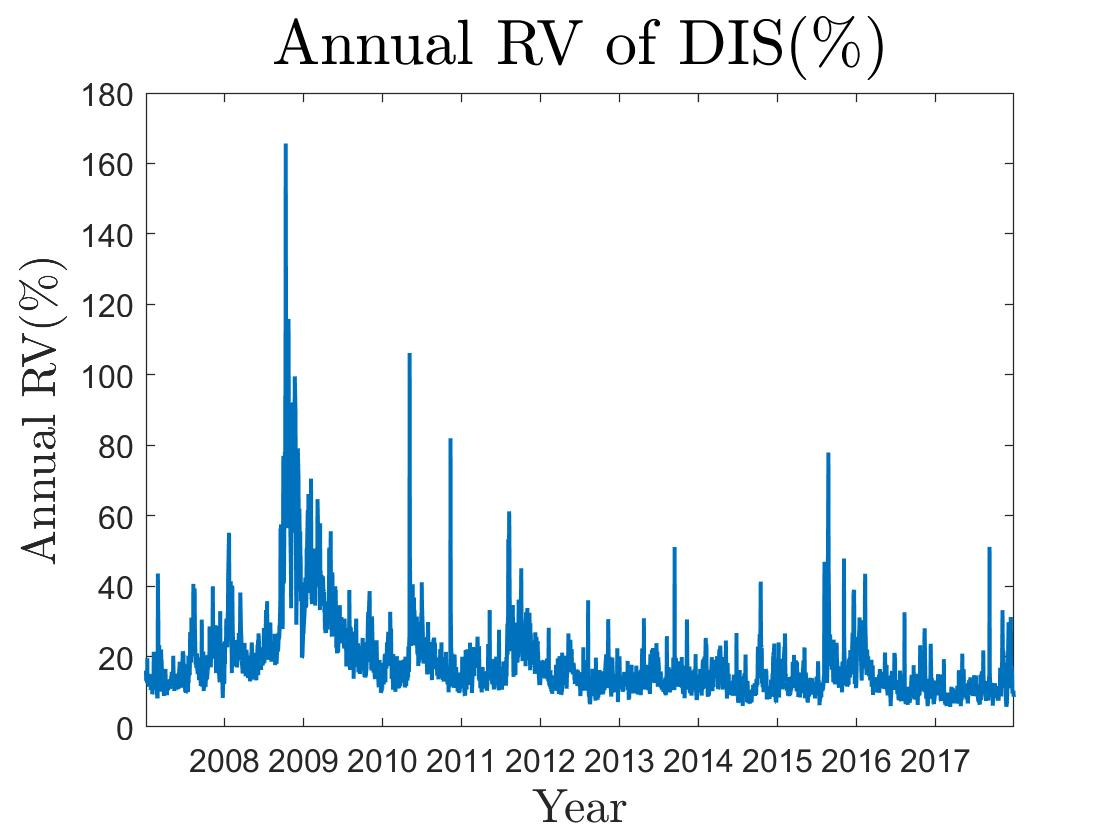
\includegraphics[width=3in]{figures/p2_ex2_a_DIS.jpg}
            \end{minipage}
            }
            \centering
            \caption{RV for PG and DIS}
\end{figure}

From the figures, the range of RV for PG and DIS are (15\%, 120\%) and (15\%,170\%) respectively. We can see that the shape of RV for both stocks are really similar: the value of RV move around 18\% and there are some fluctuations. The same as what we find in Exercise 1, the RV is abnormally high at some period. There may exist some outliers or big price jump in our data for PG and DIS.\\

The \textbf{MATLAB} code:
   \lstinputlisting{functions/realized_var.m}
   ~~\\
%----B-----
\item
Here are the figures of RV for PG and DIS:
 \begin{figure}[H]
           \subfigure{
           \begin{minipage}[l]{1\linewidth}
           \centering
             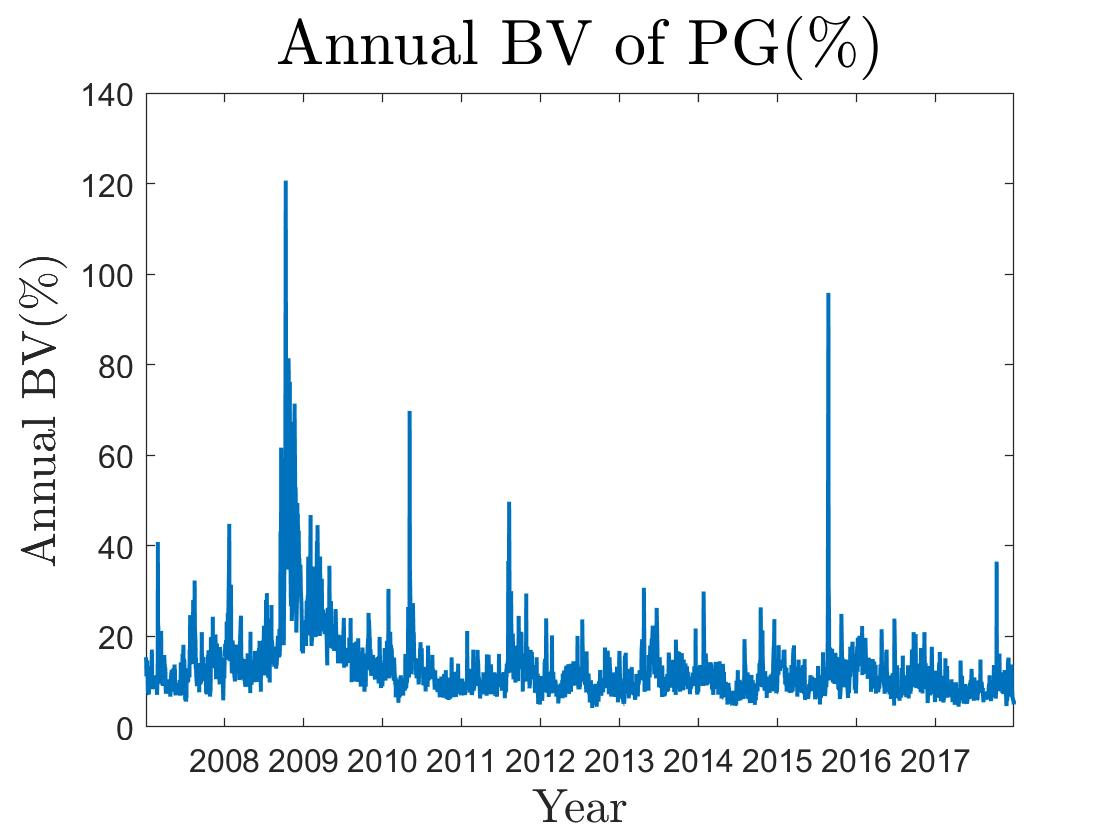
\includegraphics[width=3in]{figures/p2_ex2_b_PG.jpg}
              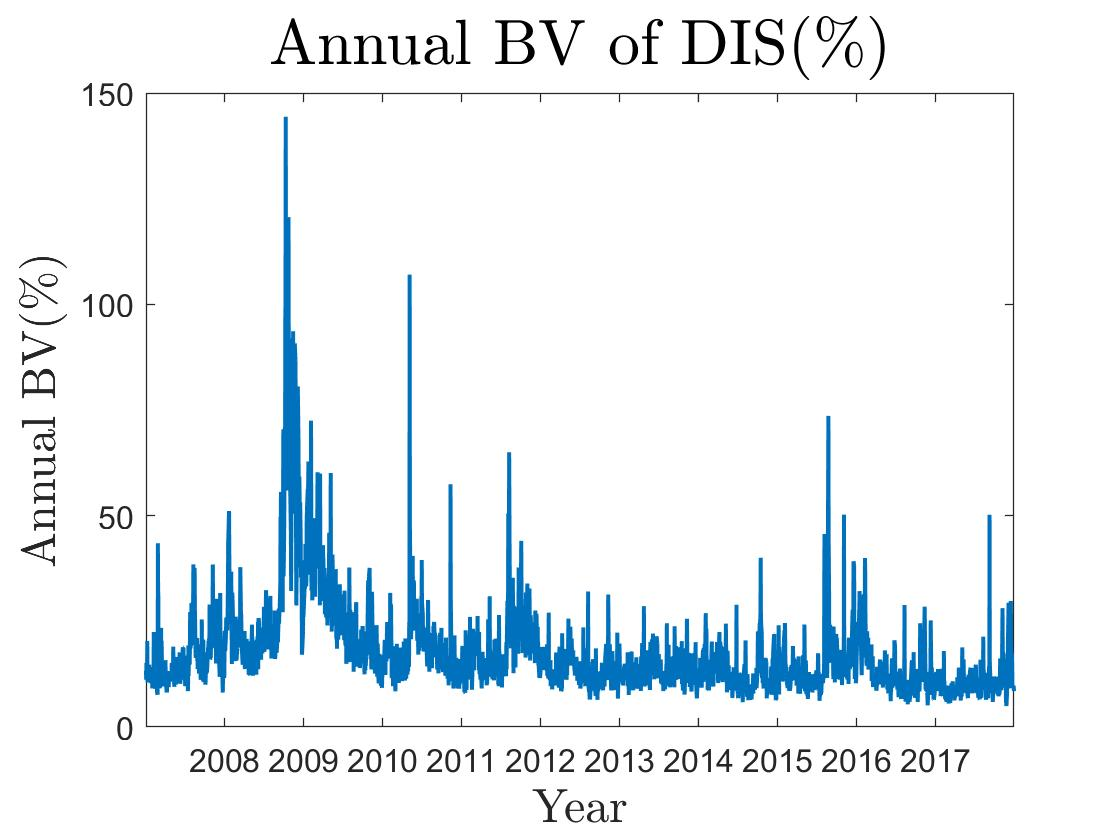
\includegraphics[width=3in]{figures/p2_ex2_b_DIS.jpg}
            \end{minipage}
            }
            \centering
            \caption{BV for PG and DIS}
\end{figure}

From the figures, the range of BV for PG and DIS are (13\%, 120\%) and (14\%,150\%) respectively. We can see that the shape of BV for both stocks are really similar: the value of RV move around 15\% and there are some fluctuations. The same as what we find in Exercise 1, the BV is abnormally high at some period. There may exist some outliers or big price jump in our data for PG and DIS.\\


The \textbf{MATLAB} code:
   \lstinputlisting{functions/bipower_var.m}
~~\\
   
%----c-----
\item
Here are the figures of RV and BV for PG and DIS:
 \begin{figure}[H]
           \subfigure{
           \begin{minipage}[l]{1\linewidth}
           \centering
             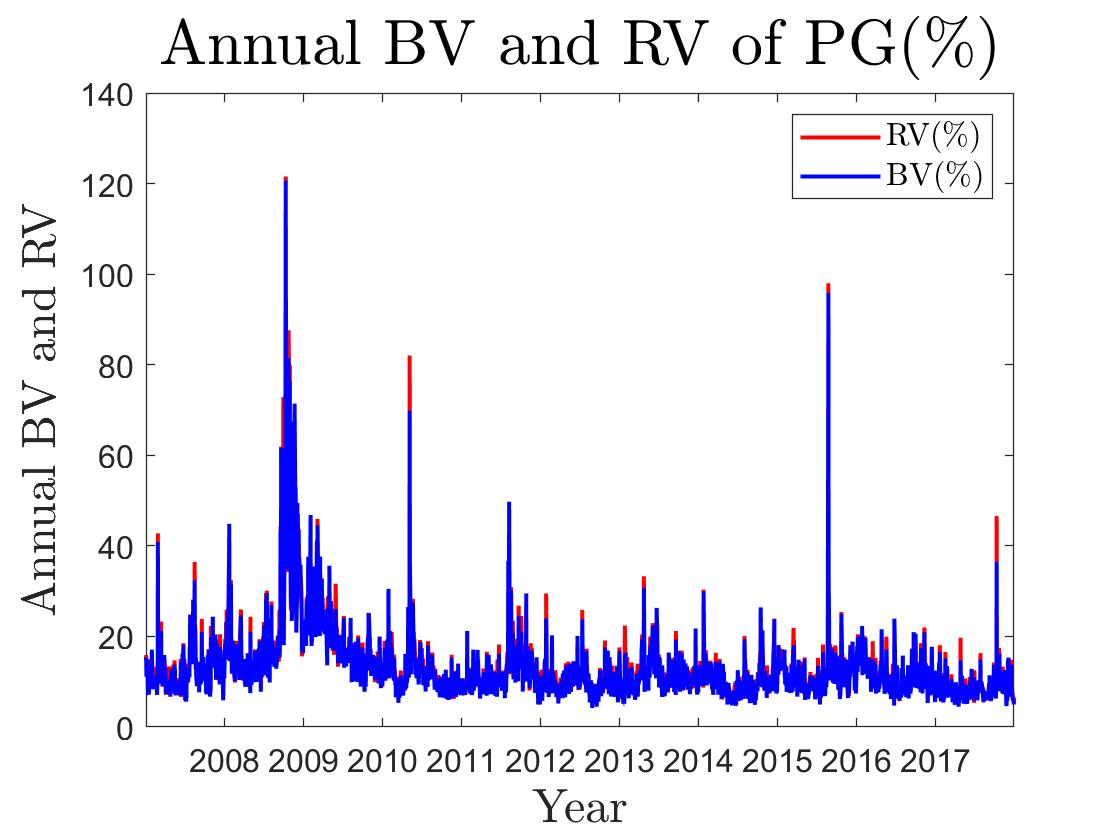
\includegraphics[width=3in]{figures/p2_ex2_c_PG.jpg}
              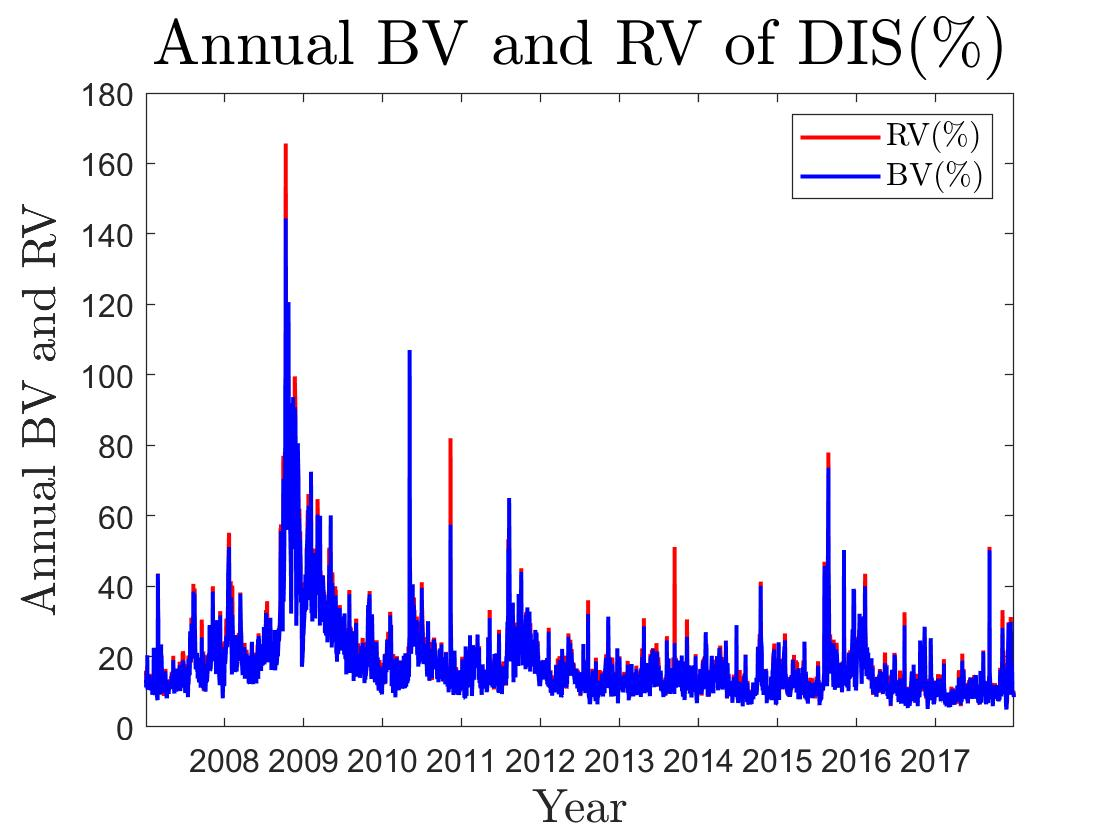
\includegraphics[width=3in]{figures/p2_ex2_c_DIS.jpg}
            \end{minipage}
            }
            \centering
            \caption{RV and BV for PG and DIS}
\end{figure}

From the figures, we can see that the shape of BV are very similar to RV for both stocks: they show the same movements. However, there are some differences between RV and BV: the value and volatility of BV is smaller than RV, this is obvious for DIS. By using BV, the max variance of DIS's log-return decrease from 170\% to 150\%. These figure show us that BV can give a smoother variance curve if our price data exists some jumps or outliers. \\
   
%----d-----
\item
Here are the figures of contribution of jumps for PG and DIS:
 \begin{figure}[H]
           \subfigure{
           \begin{minipage}[l]{1\linewidth}
           \centering
             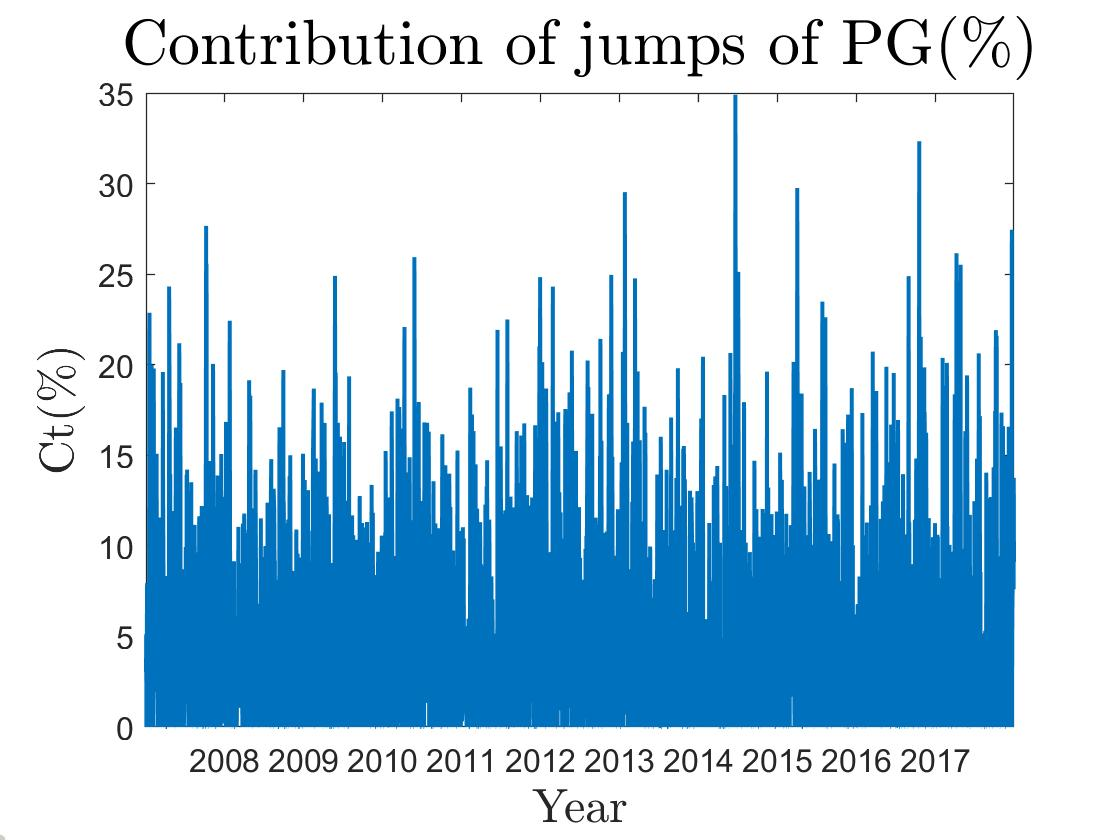
\includegraphics[width=3in]{figures/p2_ex2_d_PG.jpg}
              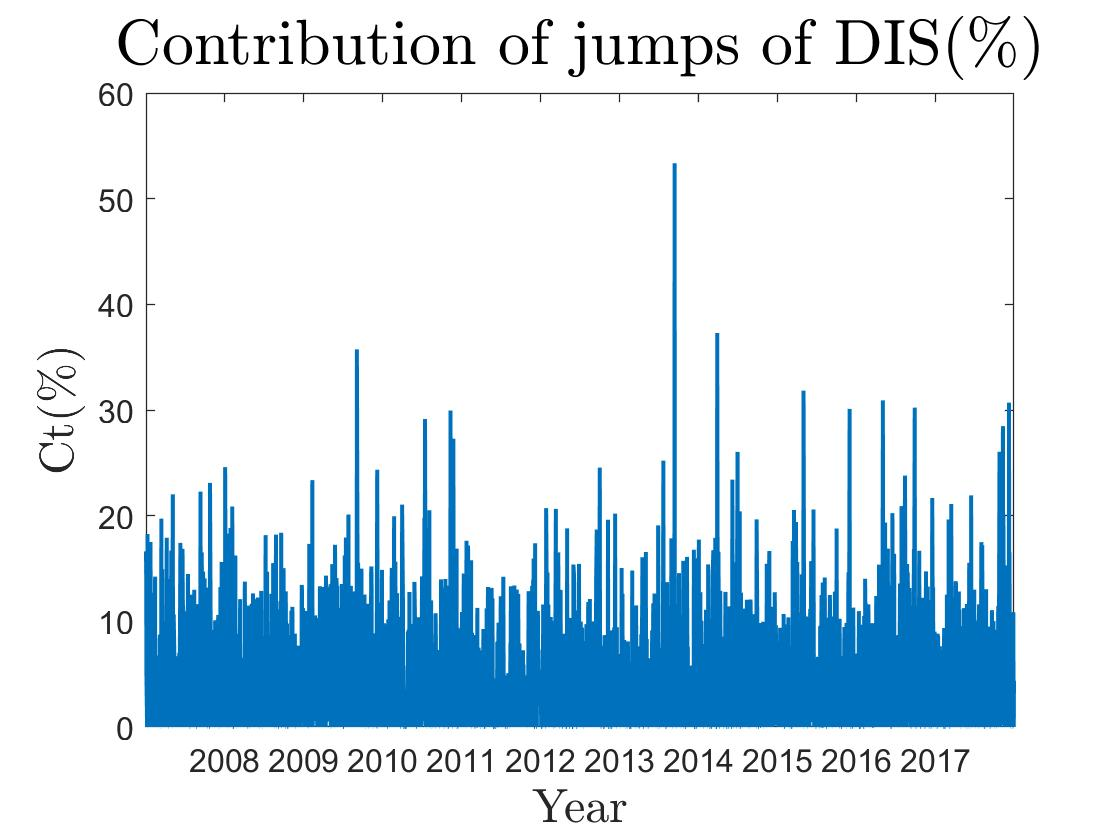
\includegraphics[width=3in]{figures/p2_ex2_d_DIS.jpg}
            \end{minipage}
            }
            \centering
            \caption{Ct for PG and DIS}
\end{figure}

From the figures, we can see that the relative contribution of jump for PG is bigger than DIS', which mean the price of PG may contains more jumps than DIS'. The mean of relative contribution of jump for PG and DIS are 4.69\% and 4.49\% respectively. These results are consistent to the finding of Huang and Tauchen in 2005: ``The empirical work indicates strong evidence for jumps, where jumps account for about 4.5\% to 7\% of the total daily variance of S\&P index, cash or futures''.\\


The \textbf{MATLAB} code for Exercise 2(here use PG as data sample):
   \lstinputlisting{scripts/p2_ex2_PG.m}
\end{enumerate}
\newpage

%---------------------------------------------
\section*{Exercise 3}
  \begin{enumerate}[label=\textbf{(\Alph*)}]
%----A-----
  \item 
  \begin{enumerate}[label=(\roman*)]
  	    \item The realized variance is a unbiased estimator for variance if the prices contain no jumps. Through using realized variance, we can treat volatility as observable by using the square of log-returns from high frequency sample to approach it.   
  	    \item The volatility signature plot is a figure to describe the relationship between average realized variance and the frequency of data sample. 
  	    \item From the volatility signature plot, we can learn that when the data frequency is extremely high, the market's microstructure noises will cause huge bias to variance. So, the sample frequency is not as highest as better, some frequency with intermediate value can let us avoid the effect of microstructure noises but provide enough data for us to estimate the variance.\\
  	    
      \end{enumerate}	
 	      
%----B-----
\item  
In 5s frequency('BAC(2015).csv') data, we have: $N=4621$ and $T=252$.\\

%----C-----
\item The follow are the volatility plot for the 1st trade day:
\begin{figure}[H]
            \centering
            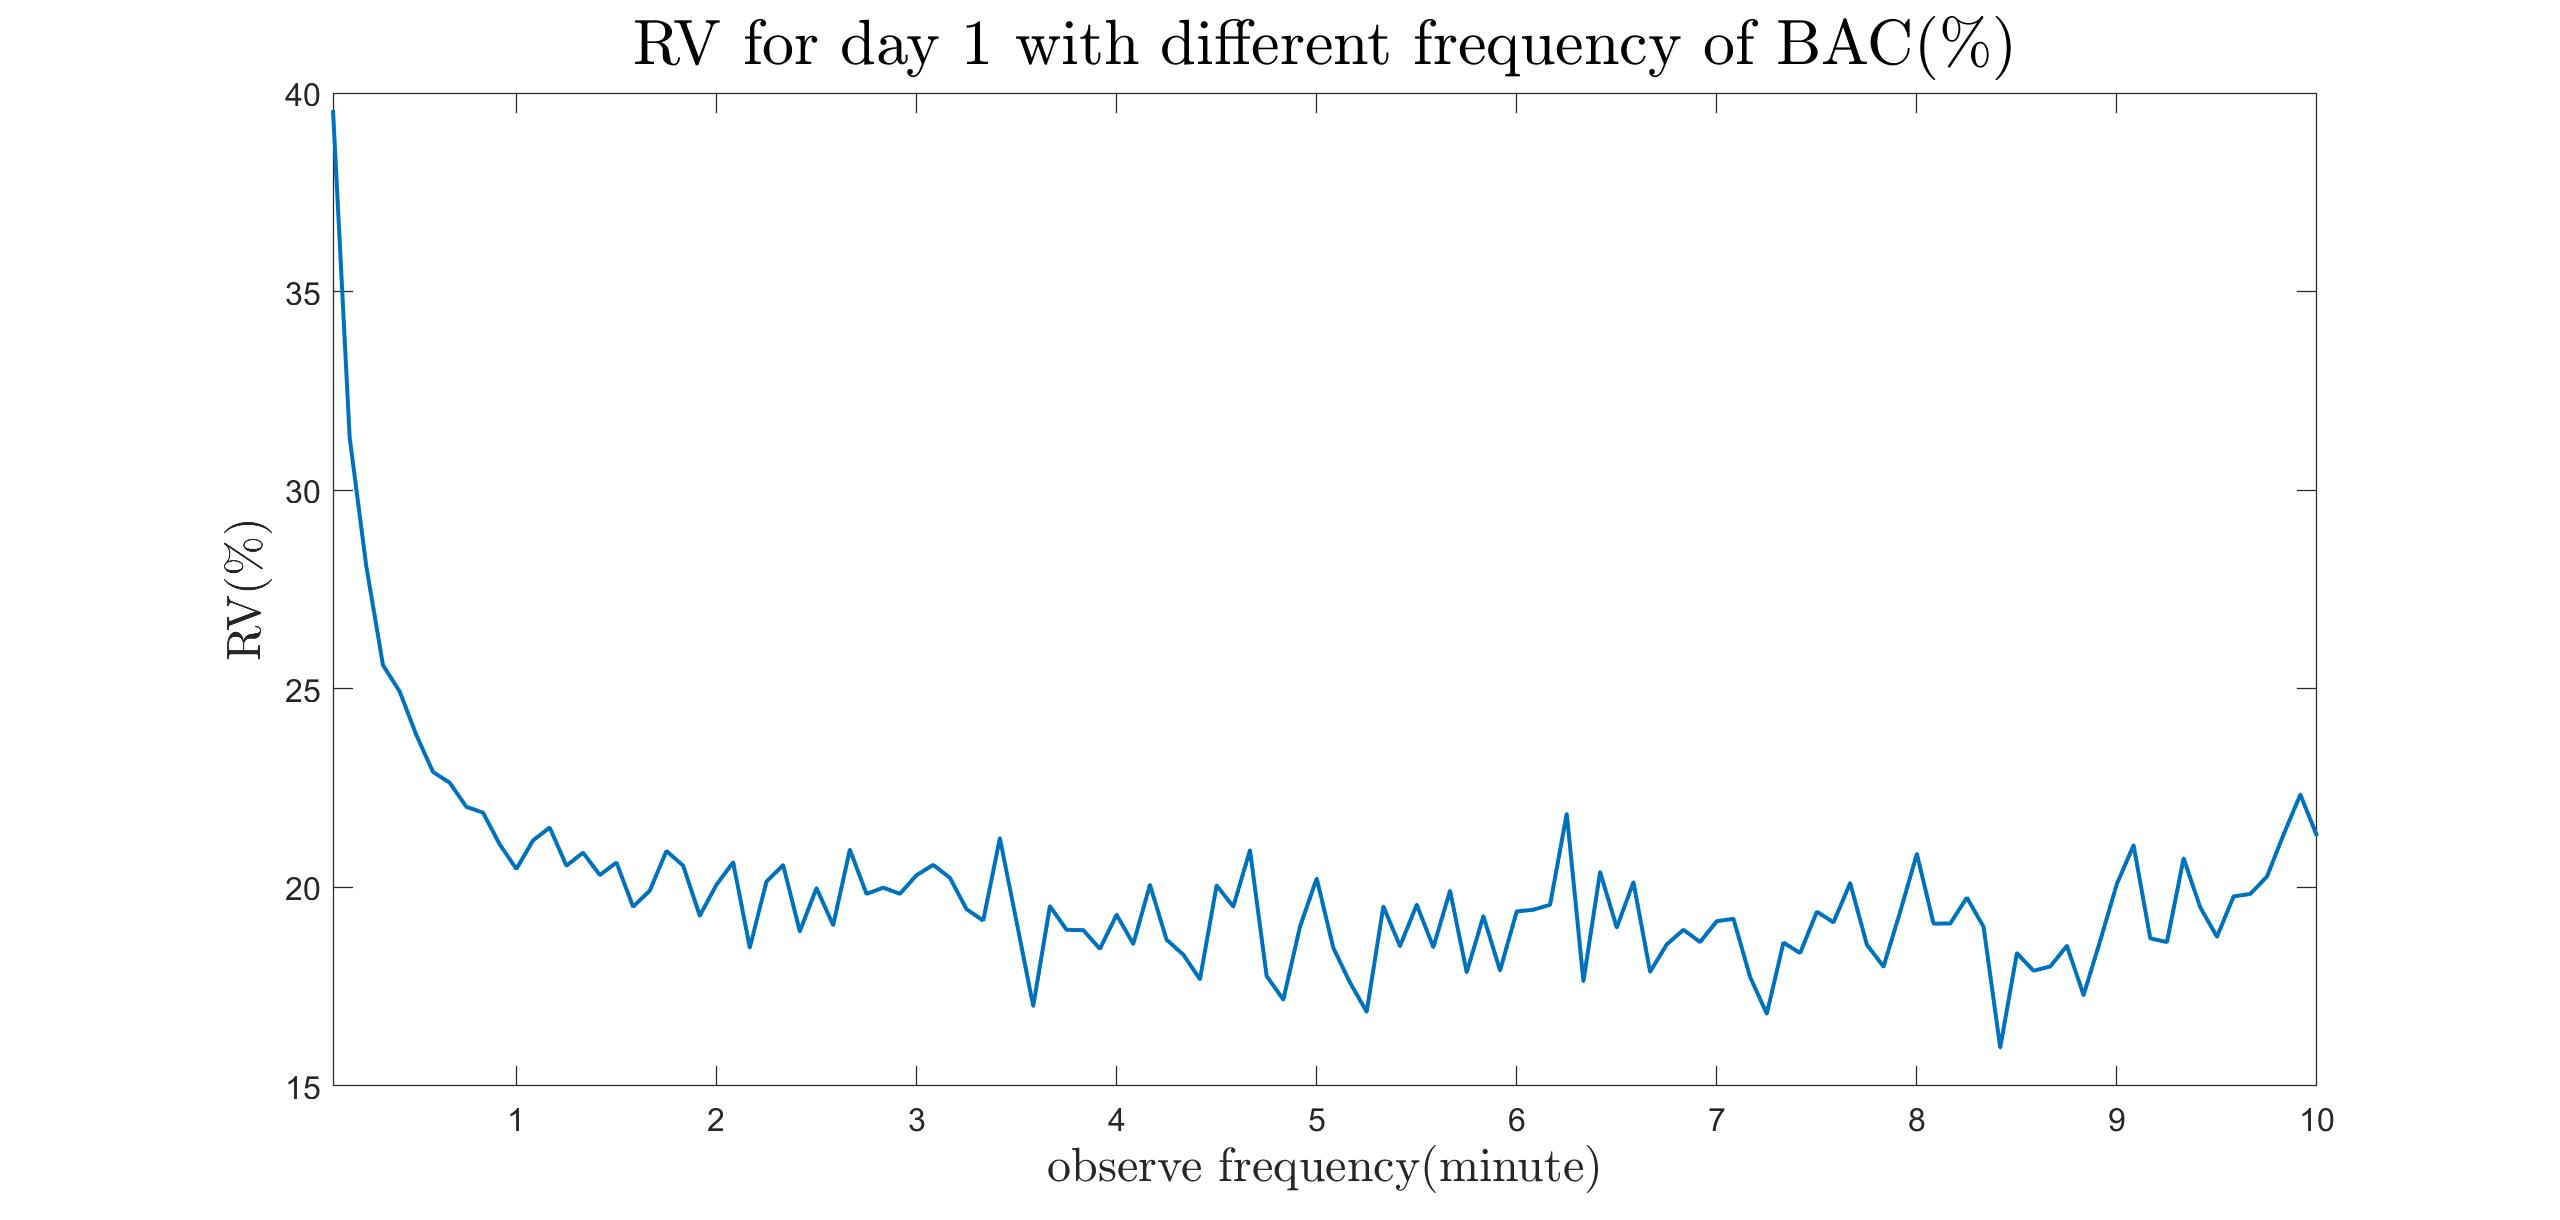
\includegraphics[width=10cm]{figures/p2_ex3_c_BAC(2015).jpg}
            \caption{RV for day1 with different frequency sample}
            \label{fig:7}
        \end{figure}
From the figure, when sample frequency is extremely high, the value of RV is extremely high, too. We can find that the value of RV first shows a down-trend and then increase when the sample frequency start decreases from 8 minute to 10 minute, which means that as the frequency of observation decreases from extremely high frequency, the volatility decreases. However, if the sample frequency is too low, say lower than 8 minute, the volatility will increase. The value of RV comes relatively stable When the frequency falls into 4 to 8 minute.  \\

%----D-----
\item The follow are the year average volatility plot:

\begin{figure}[H]
            \centering
            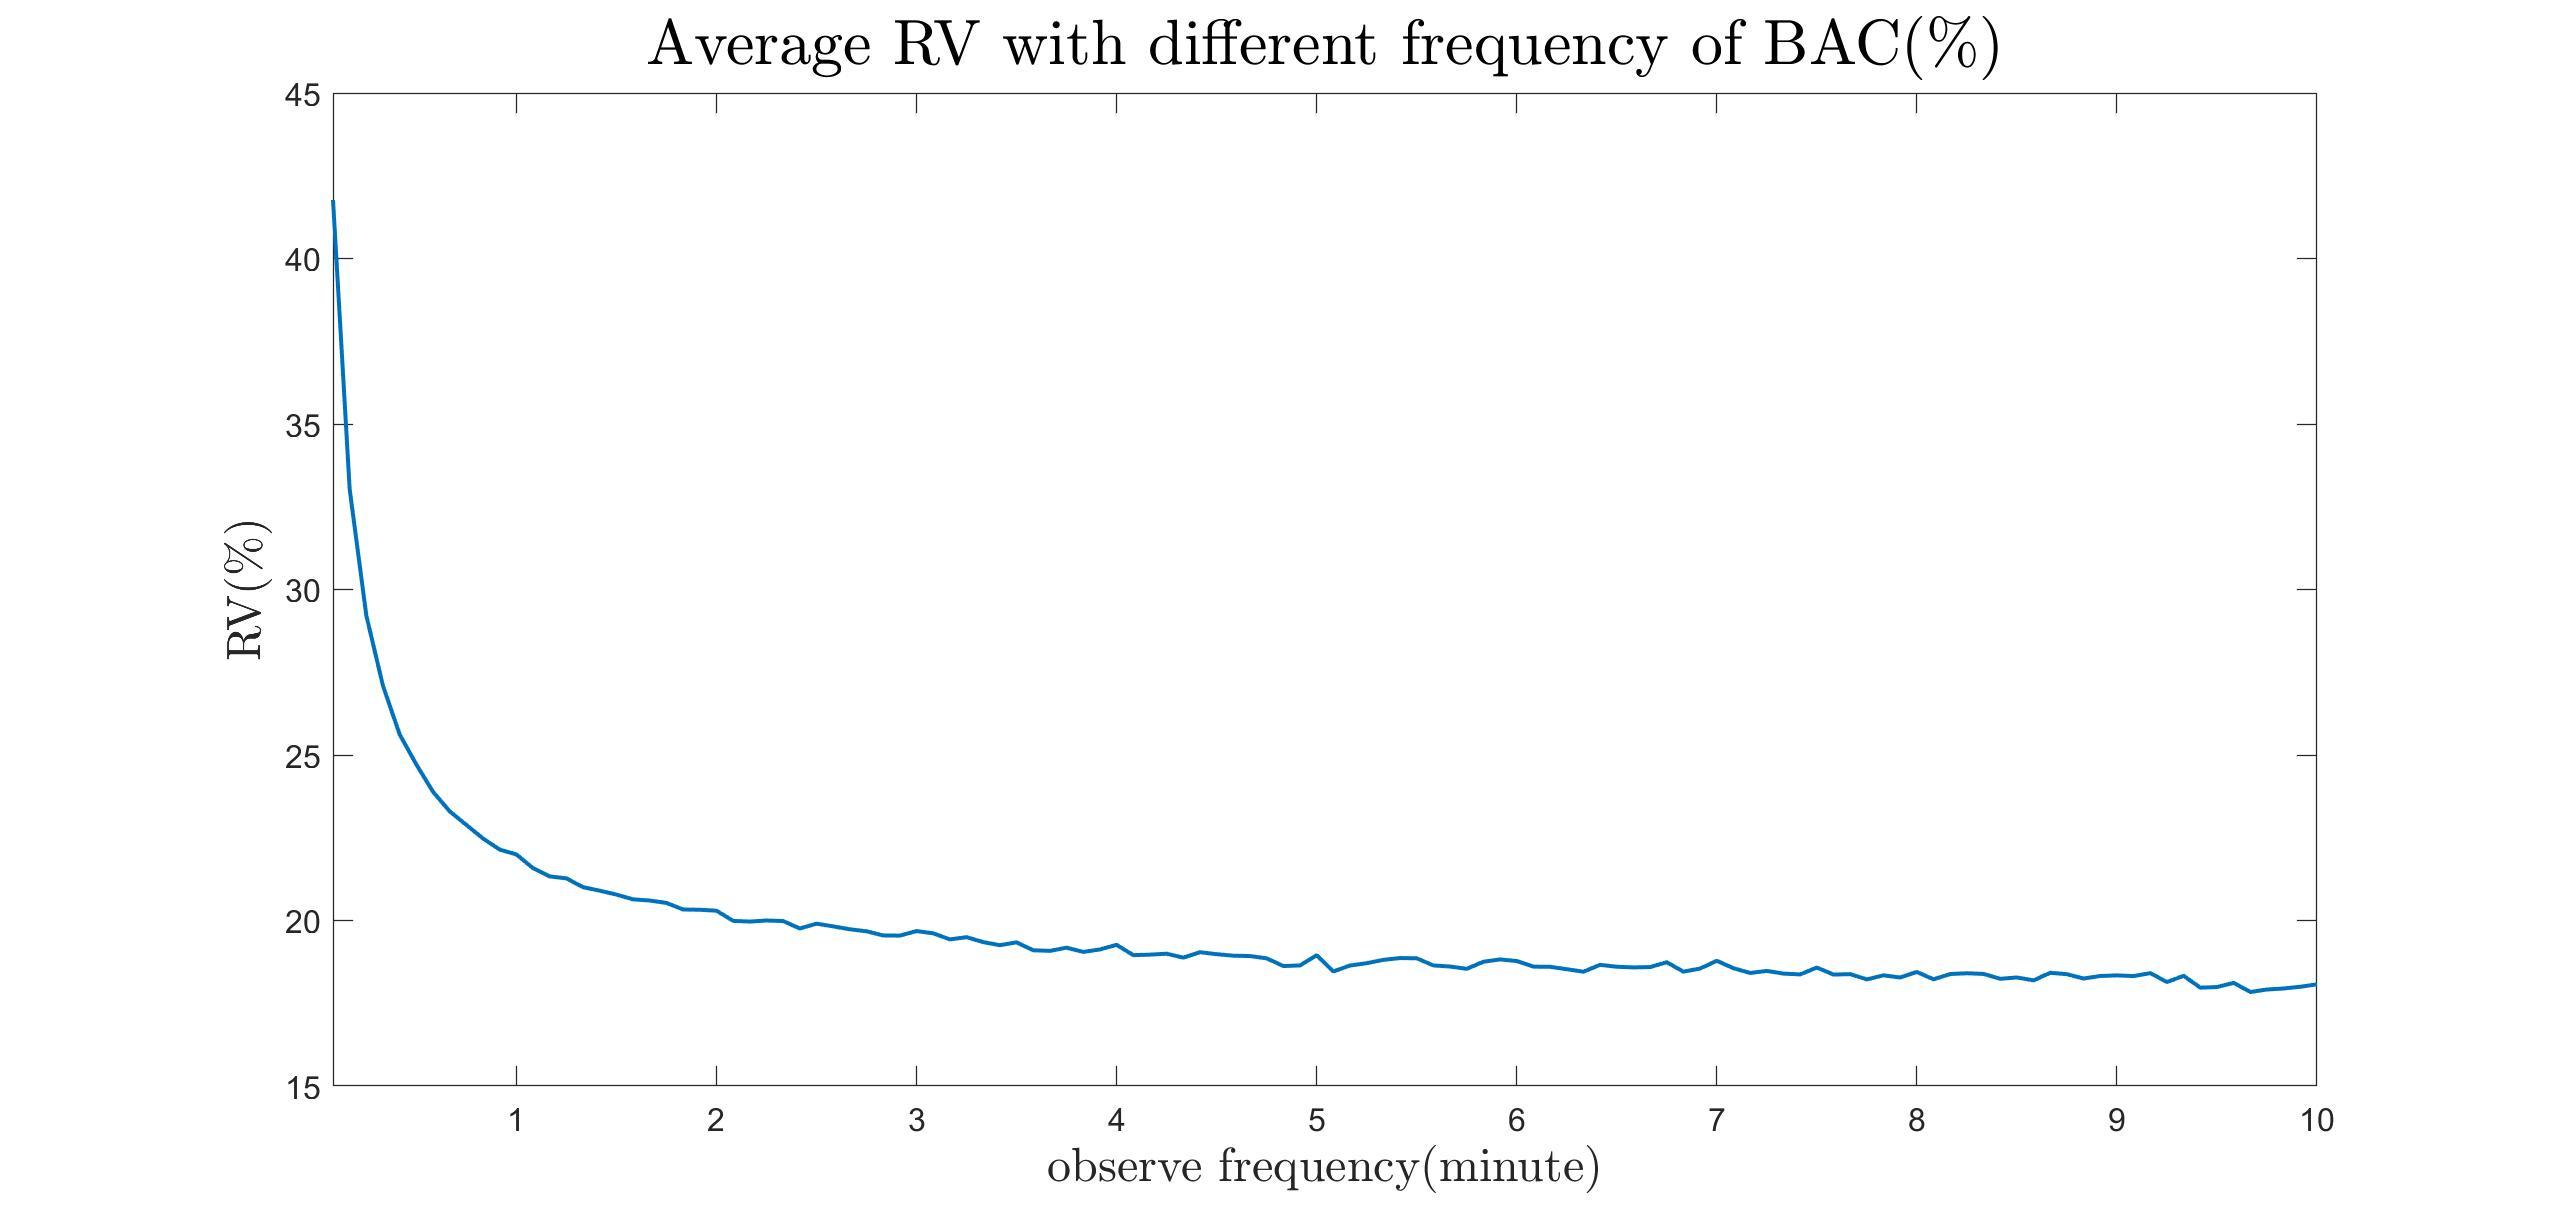
\includegraphics[width=10cm]{figures/p2_ex3_d_BAC(2015).jpg}
            \caption{Annual RV with different frequency sample}
            \label{fig:8}
        \end{figure}
From the figure, we can find that the RV curve becomes smooth as we take average for day's RV.
Same as what we find in day's RV, the value of average RV shows a down-trend, which means that as the frequency of observation decreases from extremely high frequency, the volatility decreases. However, if the sample frequency continues to decrease, the volatility will still decrease(but just a little bit). The RV value becomes stable when frequency lower than 4 minute.\\

%----E-----
\item We have construct a matrix to record the mean-difference of $RV_{J1}$ and $RV_{J2}$. According to the matrix, we find that when sample frequency is extremely high (both $J1$ and $J2$ are very small), the mean difference is large than the mean-difference of other high frequency samples. The reason may be that, since the sample is of extremely high frequency, it is of higher possibility that we will observe the noise and take it into our price data. \\

%----F-----
\item Yes. as we can see from the figure in part D, the RV curve becomes very flat. The value of RV for frequency=3 minute is 20\%, and the value of RV for frequency=8 is around 18\%. Even the fequency of observation has decreased almost two times, the value of RV just decreases by 10\%. \\

The \textbf{MATLAB} code for Exercise 3(A) to 3(F):
   \lstinputlisting{scripts/p2_ex3_BAC.m}
   \newpage
   
%----G-----
\item Here is the figure of adjusted average volatility signature plot for IBM from 2007 to 2017:
\begin{figure}[H]
            \centering
            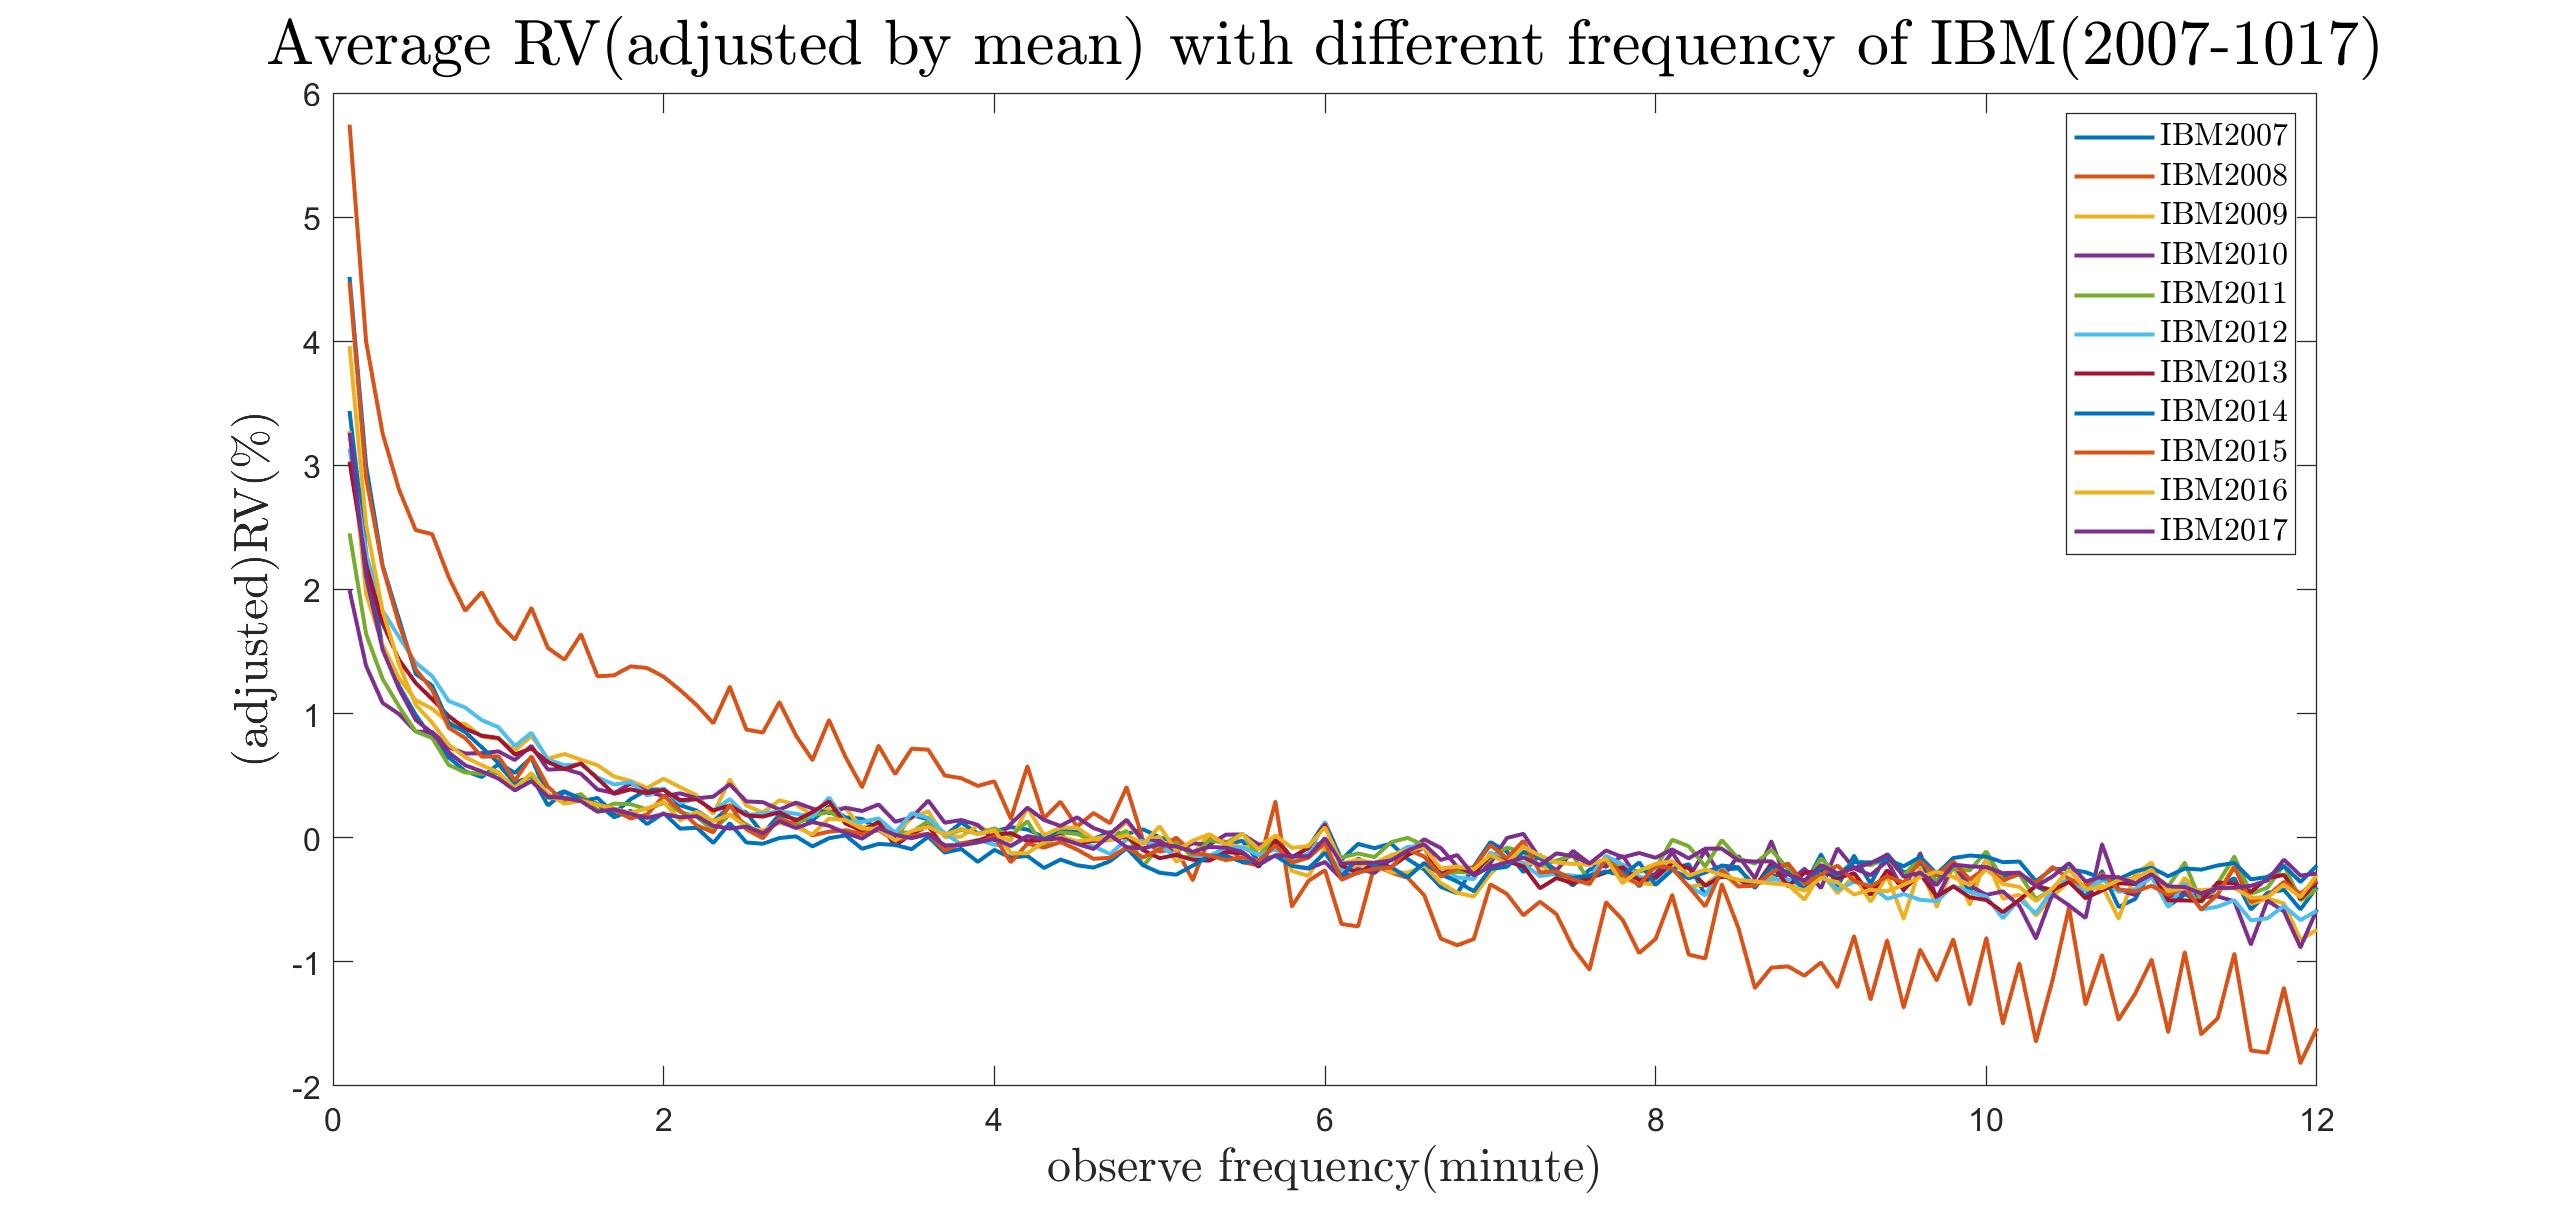
\includegraphics[width=10cm]{figures/p2_ex3_f_IBM(2007-2017).jpg}
            \caption{Annual RV with different frequency sample}
            \label{fig:9}
        \end{figure}

From the figure, for most of our sample, the adjusted average volatility curves are smooth and show a reasonable flat pattern when the frequency decreases from 3 to 8 minutes. However, for year 2008, even the year average volatility curve still has lots of fluctuations (the most volatile orange line). when the frequency decreases from 5s to 10 minutes, the volatility shows a down-trend, but it does not show a reasonable flat for sampling intervals corresponding to about 3 to 8 minutes. \\

We can see that the volatility signature plot will show a similar shape for different years. However, when there is a huge shock from the market, such as the financial crisis, the volatility signature plot will still show high volatility even we choose a ``great'' frequency for our sample.\\


The \textbf{MATLAB} code for function to calculate adjusted volatility with different frequency:
   \lstinputlisting{functions/mRV_J.m}
   \lstinputlisting{scripts/p2_ex3_f.m}
  ~~\\


\end{enumerate}
\end{document}
